\chapter{Architectures}
\label{chp:arch}

The following chapter will show and explain the different architectures used in this thesis.
The architectures were based on existing architectures used in the automotive industry as well as experimental ones based on certain attributes.

While architectures used in the automotive industry are complex, with sometimes up to 150 ECUs in one model, 
the architectures used in this thesis were sized down to a more manageable size, with 20 ECUs for each architecture.
Each architecture was modeled using these components:

\begin{itemize}

    \item \textbf{ECUs}: The different ECUs in the architecture. They are the nodes of the graph.
    
    \item \textbf{Entry points}: The entry points to the architecture. The only possible entries are the external interfaces that an ECU might have.
    
    \item \textbf{Targets}: ECUs that are considered targets for an attacker. They are targets because they contain sensitive data or because they are critical for the vehicle's functionality.
    
    \item \textbf{Bus systems}: ECUs are connected to each other using bus systems. The bus systems are the edges in the graph. The possible bus systems are \textit{CAN, CANFD, LIN, FlexRay, MOST} and \textit{Ethernet}.
    
    \item \textbf{Interfaces}: The interfaces are the connections between the ECUs and the external world. They are the connections between the ECUs and the bus systems. The possible interfaces are \textit{Bluetooth, WiFi,} and \textit{GNSS}.
    
    \item \textbf{Attack feasibility}: Each component of the architecture (ECU, bus system, interface) has its own rating for its attack feasibility.

\end{itemize}

\section{Components}
\label{sec:components}

Using the scale mentioned in \ref{sec:config} for each component, a higher rating means that the component is more secure, i.e. might have more security mechanisms in place,
while a lower rating means that the component lacks such mechanisms.
This also indicated that the higher the overall score one architecture receives, the more secure it is.
This subsection will further explain some the aforementioned components as well as their attack feasibility based on their attributes.

\begin{itemize}
    \item \textbf{\gls{ecu}}: An ECU is an embedded system in an automotive system that cotrnols various systems in the vehicle.
    ECUs are typically connected to each other using a bus system, enabling communication between the each other.
    Since each ECU has an individual task, whose criticality varies, the attack feasibility of an ECU is based on the criticality of the task it performs.
    Thus, each ECU will have an own attack feasibility. 
    For example, the Engine Control Unit (ECU) is responsible for the engine, and thus is a critical ECU, 
    whereas the SEAT ECU, that are responsible for the seats in a vehicle, are not as critical.
    Over the years, vehicles have become more and more complex, and thus the number of ECUs has increased.
    
    \item \textbf{\gls{can}}: CAN a communication protocol utilized in modern vehicles and industrial applications 
    to enable devices and microcontrollers to communicate with one another. 
    It was developed by Bosch in the 1980s and has since become a widespread standard for in-vehicle communication.
    It is a dependable, durable, and cost-effective communication protocol that has become an indispensable component of modern vehicle electronics.
    Since the \gls{can} bus is the most common bus system used in a vehicle, it will be set as a base line for security in this thesis.

    \item \textbf{\gls{canfd}}: It is an extension of \gls{can} bus.
    It provides higher data transfer rates, more efficient data communication, and increased bandwidth compared to the original \gls{can} bus.
    It is backward compatible with the original CAN bus, which means it can function on the same network as older CAN devices.
    In terms of security it will be rated a bit higher than \gls{can}.
    Modern implementations of both protocols incorporate security features, such as message authentication and encryption.
    
    \item \textbf{\gls{flexray}}: It is a bus system that is used in the automotive industry used to facilitate high-speed real-time communication.
    It was developed by a group of automotive companies and aims to meet the growing need for real-time communication in complex automotive systems.
    FlexRay is utilized to link ECUs requiring high bandwidth, such as advanced driver-assistance systems and safety-critical systems. 
    It ensures deterministic data transfer, delivering data at predetermined intervals with a guaranteed maximum latency. 
    This is crucial for safety-critical systems that rely on fast and dependable data transfer.
    FlexRay is designed for use in safety-critical systems and provides deterministic data transfer, making it highly reliable and resistant to interference. 
    It also supports encryption and authentication, providing additional security features.

    \item \textbf{\gls{lin}}: LIN is a communication protocol used to connect and communicate with low-speed peripherals in modern vehicles and other industrial applications. 
    It is a lower-cost alternative to the CAN bus communication protocol, developed by a group of automotive companies 
    and generally considered to be less secure than other protocols, as it doesn't support encryption or authentication
    LIN is weaker bus system than \gls{can} and \gls{canfd}, in terms of technology but also use, which will contribute to the rating.
    
    \item \textbf{\gls{most}}: It is a communication protocol that enables high-bandwidth multimedia data transfer between devices in modern vehicles. 
    It was developed by a consortium of automotive and multimedia companies and offers high-speed, dependable, and cost-effective data transfer.
    It is a highly dependable communication protocol that has gained increase popularity in the automotive industry and
    provides secure communication between devices through encryption and authentication

    \item \textbf{Ethernet}: Ethernet is a wired networking technology that enables the transfer of data between computers and devices within a local area network (LAN)
    It delivers fast, secure, and reliable data transfer, which makes it ideal for a variety of applications such as internet connectivity, file sharing, and multimedia streaming.
    Ethernet is commonly used in modern vehicles for connecting various devices, including infotainment systems, sensors, and advanced driver-assistance systems. 
    It is a crucial part of modern automotive systems, providing dependable and swift data transfer for various applications, however, it is also expensive and complex to implement.
    While it is vulnerable to physical attacks, such as cable tapping, it is generally considered to be more secure than wireless technologies.

    \item \textbf{Bluetooth}: Bluetooth is a wireless technology used to exchange data between electronic devices over short distances.
    In modern vehicles, Bluetooth is used for hands-free phone calls, music streaming, and other features that require wireless connectivity. 
    It has become an essential component in modern automotive systems, providing a convenient and safe way for drivers to interact with their vehicles.
    Though uses encryption to secure the communication between devices, but vulnerabilities have been discovered in the past that allow attackers to intercept and decrypt Bluetooth traffic

    \item \textbf{WiFi}: WiFi is a wireless communication technology that enables electronic devices to connect to the internet and exchange data wirelessly over a local area network (LAN)
    It uses radio waves to transmit data between devices, typically using the 2.4GHz or 5GHz frequency bands.
    In modern vehicles, WiFi is used for a variety of applications, such as infotainment systems, navigation, and telematics. 
    It enables passengers to access the internet, stream video content, and browse the web, enhancing the in-car entertainment experience. 
    WiFi also provides a means for vehicles to communicate with other devices, such as smartphones or smart home devices, to access remote services or home automation features.
    Though it has improved in terms of security over the years, is vulnerable to various attacks, including weak encryption, insecure network configurations, and attacks on the wireless network itself.

    \item \textbf{\gls{gnss}}: GNSS is a satellite-based navigation technology that can determine precise positioning and timing information anywhere on Earth. 
    It comprises various satellite navigation systems, such as GPS, GLONASS, Galileo, BeiDou, and other regional systems.
    GNSS uses a constellation of satellites orbiting the Earth to provide accurate location and timing data to receivers on the ground. 
    These receivers analyze signals from the satellites to determine their position and velocity, making it possible to navigate precisely over long distances.
    GNSS is used in vehicles primarily for navigation purposes.
    It is generally considered to be the most secure technology since it is difficult to intercept and manipulate signals from GNSS satellites, 
    and modern receivers incorporate security features to mitigate the risk of attacks.
\end{itemize}
    
Ranking these technologies in terms of security is a complex task, as each technology works differently,
has different use cases and different security characteristics and vulnerabilities.
However, based on experts' experience, these values were given each component:

\begin{table}[h]
    \centering
    \begin{tabular}{|l|c|}
    \hline
    \textbf{Technology} & \textbf{Feasibility Rating} \\
    \hline
    CAN & 0.5 \\
    CANFD & 0.6 \\
    FlexRay & 0.9 \\
    LIN & 0.1 \\
    MOST & 0.3 \\
    Ethernet & 0.8 \\
    Bluetooth & 0.4 \\
    WiFi & 0.4 \\
    GNSS & 0.8 \\
    \hline
    \end{tabular}
    \caption{Ranking of automotive communication technologies based on security}
\end{table}

Note: the higher the rating, the more secure the technology is.

\section{Training set architectures}
\label{sec:trainingarch}

Ten architectures were used as a "training set" to determine and calibrate the criteria used to 
evaluate the remaining architectures, which are the focus of the comparison.
This was done to avoid biasing the results, as well as have a well evaluated criteria.
In addition, the training set is much larger than the main set, thus the results are more accurate.

The following section will describe the test architectures and estimate the expected behavior of the architectures.

\subsection{Architecture 1}
\label{subsec:arch1}

\begin{figure}[h!]
    \caption{Architecture 1}
    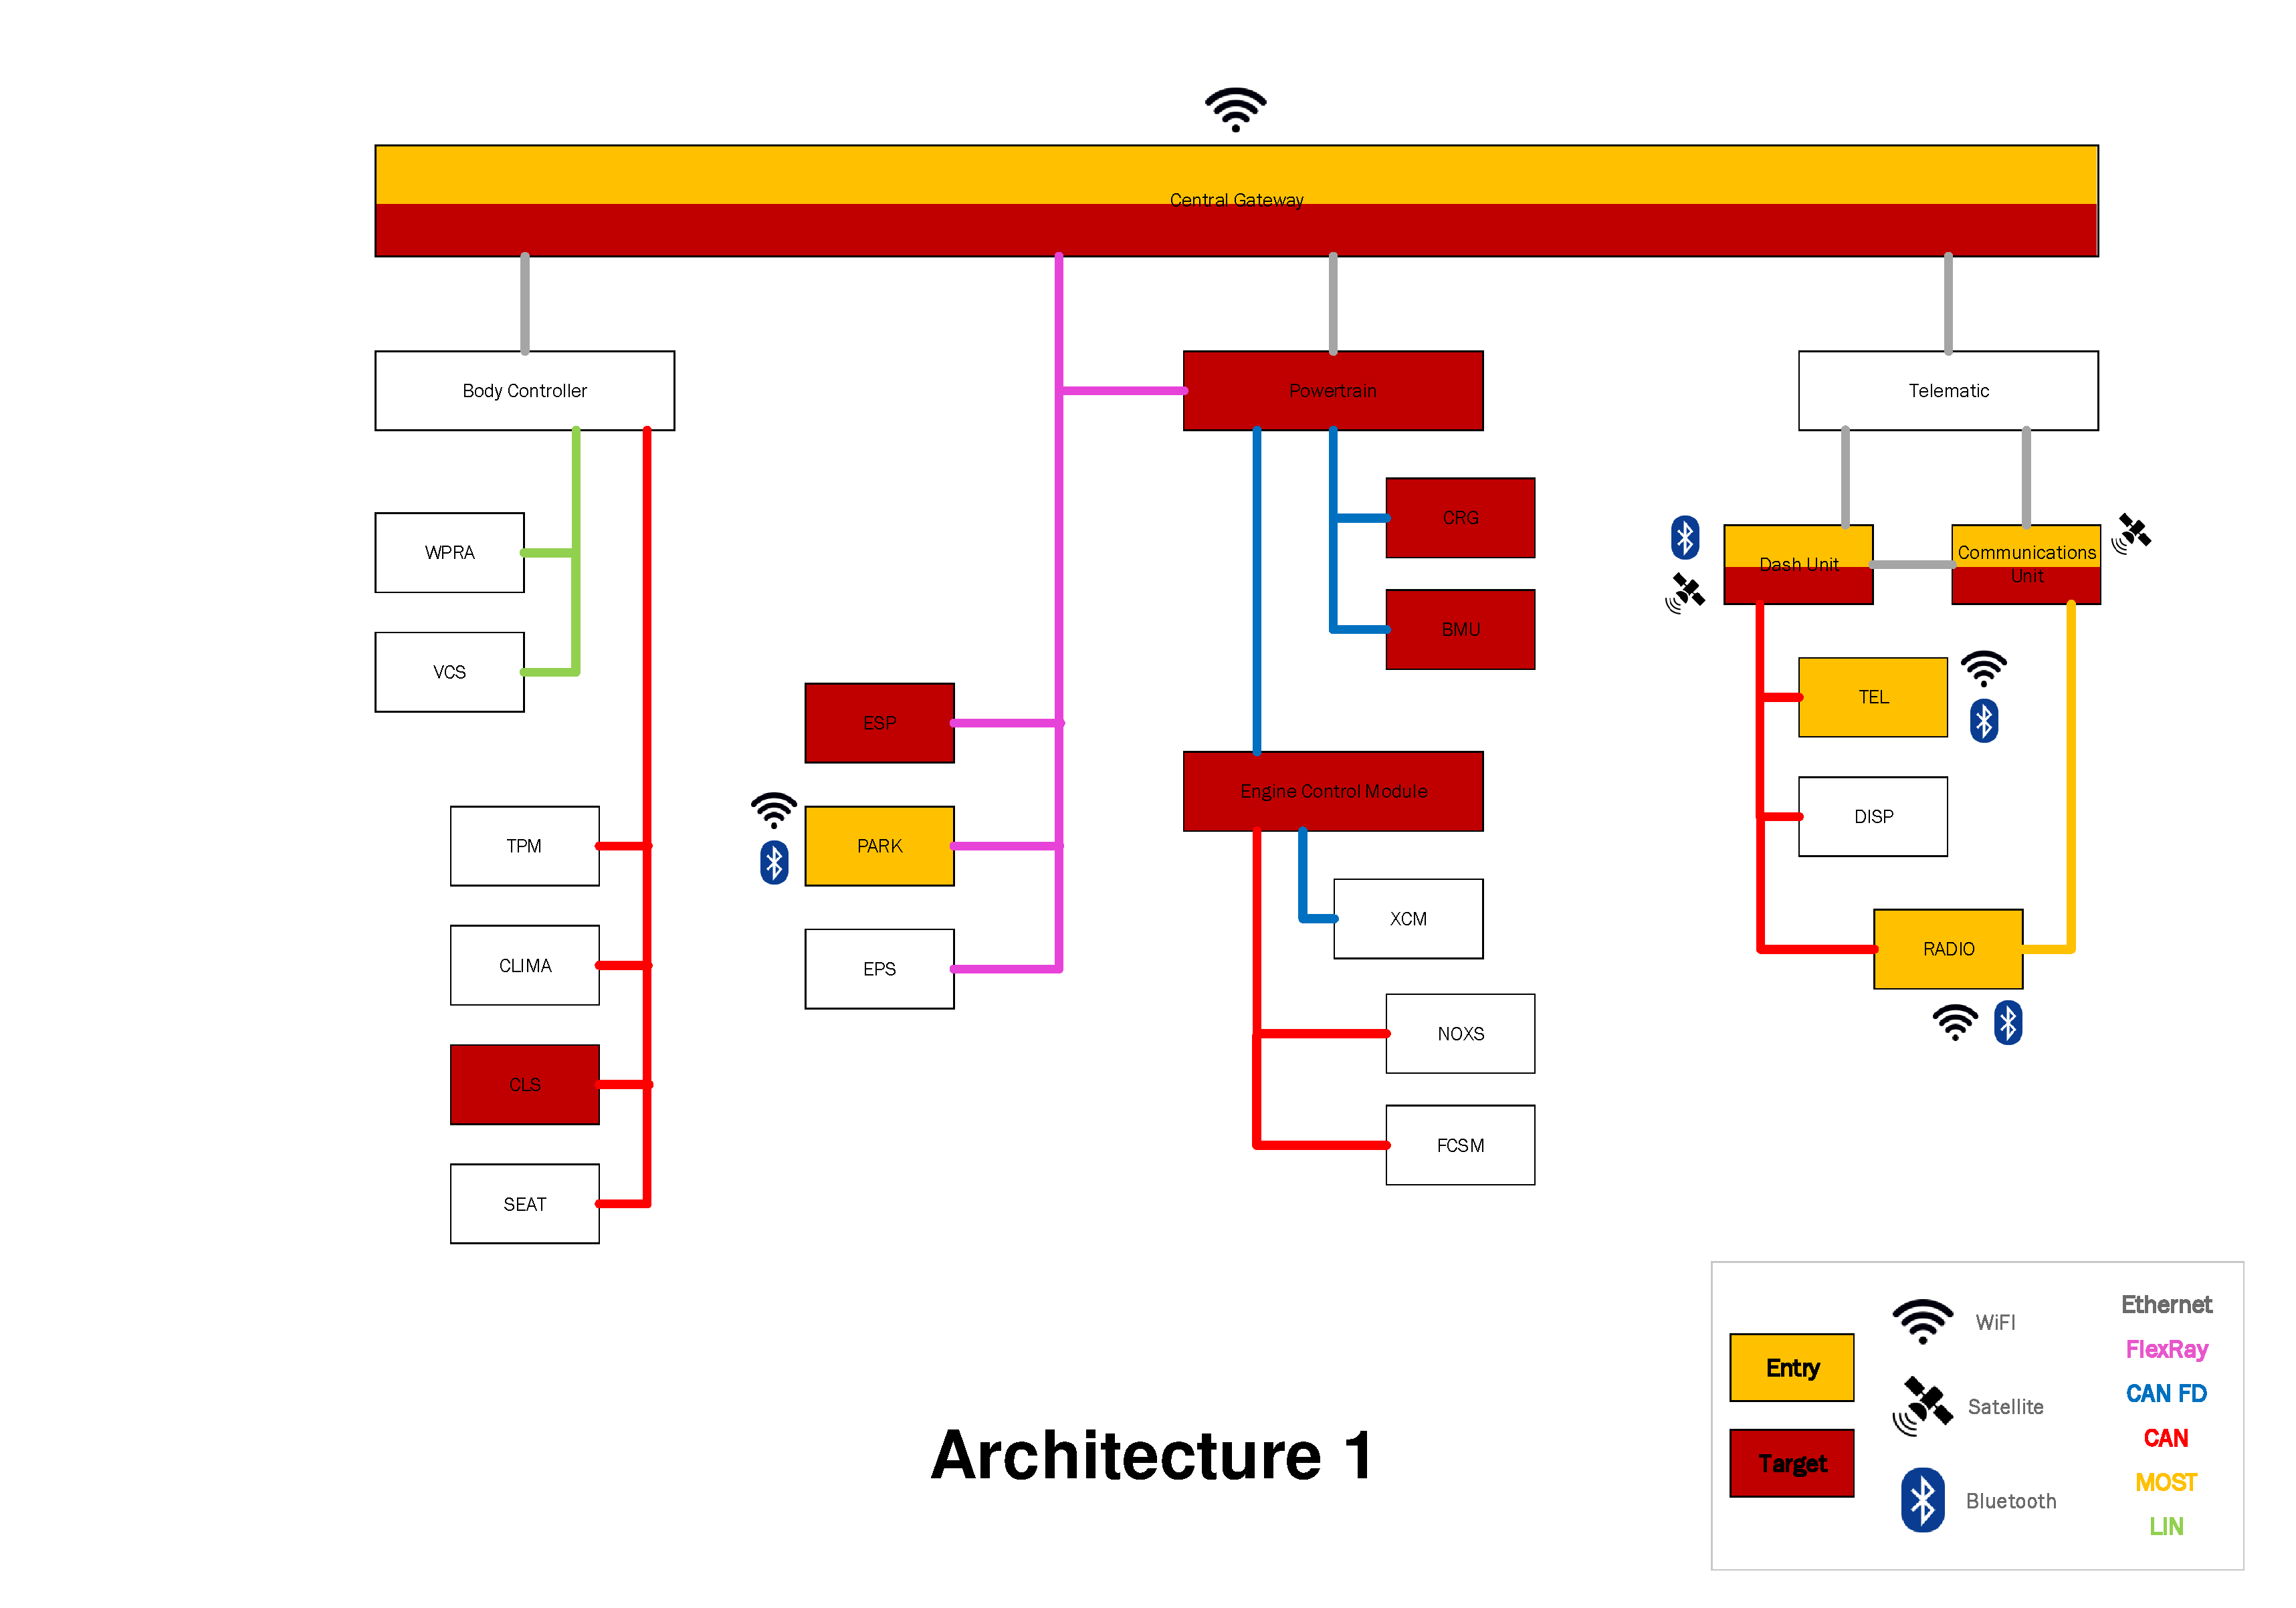
\includegraphics[width=\textwidth, page=1]{../Architectures-survey.pdf}
\end{figure}

Architecure 1 represent the most realistic architecture, as it is modeled after an actual architecture used in the automotive industry.
It was important to include this architecture, since it could offer valuable insight into the real world.
The first architecture offers six entry points with three being targets, one of it even being the \textit{Central Gateway}, and eight targets in total.
\par


\subsection{Architecture 2}
\label{subsec:arch2}	

\begin{figure}[h!]
    \caption{Architecture 2}
    \includegraphics[width=\textwidth, page=2]{../Architectures-survey.pdf}
\end{figure}

Architecure 2 is essentially the same as architecture 1, but without a central gateway, 
so we could see how the architecture would perform without it.\par


\subsection{Architecture 3}
\label{subsec:arch3}

\begin{figure}[h!]
    \caption{Architecture 3}
    \includegraphics[width=\textwidth, page=3]{../Architectures-survey.pdf}
\end{figure}

The idea of architecture 3 was to group all the entry interfaces, to see how a centralized entry would affect the architecture.
Isolating the possible entry locations reduces the attack surface, prolongs the attack path to each target, and increases the number of ECUs used for the path, thus making the attack more difficult as the attacker would have to compromise more ECUs.\par


\subsection{Architecture 4}
\label{subsec:arch4}

\begin{figure}[h!]
    \caption{Architecture 4}
    \includegraphics[width=\textwidth, page=4]{../Architectures-survey.pdf}
\end{figure}

Architecture 4 offers entry points from all domain controllers, however notice how every domain controller only has one type of interface.
In addition, ECUs that rely on more than one interface would now need to use that interface from another ECU.
For example, \textit{TEL} has to use the Bluetooth interface of the \textit{Body Controller} instead of its own Bluetooth interface.
Having an entry point from each domain controller enlargens the attack surface, as the attacker would only need to compromise one ECU in each domain controller to gain quick access to the whole domain.\par


\subsection{Architecture 5}
\label{subsec:arch5}

\begin{figure}[h!]
    \caption{Architecture 5}
    \includegraphics[width=\textwidth, page=5]{../Architectures-survey.pdf}
\end{figure}

Architecture 5 uses only Ethernet as the bus system, to see how the architecture would perform without any other bus system.
Ethernet was chosen because it recieves the securest attack feasibility rating.
In addition, there has been a trend in the automotive industry to increasingly use Ethernet as the bus system and maybe even some day replace most of the traditional CAN bus system.\par


\subsection{Architecture 6}
\label{subsec:arch6}

\begin{figure}[h!]
    \caption{Architecture 6}
    \includegraphics[width=\textwidth, page=6]{../Architectures-survey.pdf}
\end{figure}

Architecture 6 puts all the ECUs onto an own bus system.
This is interesting, as the possible ECUs on a bus are limited to just one, thus many of the attack paths and number of ECUs used for the path are trimmed down to a few.
\par


\subsection{Architecture 7}
\label{subsec:arch7}

\begin{figure}[h!]
    \caption{Architecture 7}
    \includegraphics[width=\textwidth, page=7]{../Architectures-survey.pdf}
\end{figure}

Architecture 7 has a similar idea to architecture 6, but instead of putting all the ECUs on their own bus system, it puts all the ECUs that used the same bus system on the same bus system.
Now, the feasibility of the bus rating is much more significant to the overall architecture rating and can indicate whether the used bus systems are secure enough.\par



\subsection{Architecture 8}
\label{subsec:arch8}

\begin{figure}[h!]
    \caption{Architecture 8}
    \includegraphics[width=\textwidth, page=8]{../Architectures-survey.pdf}
\end{figure}

Architecture 8 only has one entry point, namely the \textit{Central Gateway}. 
This architecture eliminates other entry points meaning the attack paths all start at the same point, thus reducing the attack surface.
Additionally, the feasibility rating of the interfaces is more significant than before and the attack paths might become much more linear, thus the feasibility rating of the components themselves becomes a greater factor.\par


\subsection{Architecture 9}
\label{subsec:arch9}

\begin{figure}[h!]
    \caption{Architecture 9}
    \includegraphics[width=\textwidth, page=9]{../Architectures-survey.pdf}
\end{figure}

Architecture 9 is essentially the same as Architecture 4, but without a central gateway.
Again, the entry points are more dispersed resulting in an enlarged attack surface \par


\subsection{Architecture 10}
\label{subsec:arch10}

\begin{figure}[h!]
    \caption{Architecture 10}
    \includegraphics[width=\textwidth, page=10]{../Architectures-survey.pdf}
\end{figure}

The final architecture of the test set only includes one of each interfaces but more dispersed than that of architecture 8.
Note that the entries are also grouped together which shares the same idea of architecture 3.\\
